\documentclass[10pt]{article}

    

\def\Type{LessonCaelan}
\newcommand\TypeNum{Lesson 1}
\newcommand\TypeTitle{Slopes \& Rates of Change \\ Key}
\newcommand\Semester{Fall 2021} %Not Used 
\newcommand\Course{MATH 1190 \& 1210}
\newcommand\Targets{{\bf\color{ProcessBlue}F1}}

\usepackage{preambleDJ} 

%%%%%%%%%%%% BEGIN DOCUMENT %%%%%%%%%%%%%%%
%%%%%%%%%%%% BEGIN DOCUMENT %%%%%%%%%%%%%%%
%%%%%%%%%%%% BEGIN DOCUMENT %%%%%%%%%%%%%%%
%%%%%%%%%%%% BEGIN DOCUMENT %%%%%%%%%%%%%%%
%%%%%%%%%%%% BEGIN DOCUMENT %%%%%%%%%%%%%%%

\begin{document}
\pagestyle{otherpages}
\thispagestyle{firstpage}

\vs{0.5}


\textbf{Intended Learning Targets}
After this lesson, you will be able to 

\begin{itemize}
    \item Find and distinguish the net change and average rate of change. (\target{F1})
    \item Interpret the average rate of change graphically as the slope the respective linear function. (\target{F1})
\end{itemize}

\vspace{-0.5cm}

\hrulefill

\vspace{0.5cm}

{\bf\color{blue}Warm-up }\exercise{\bf\color{ProcessBlue}F1}Respond to the following prompts.\\
    \begin{enumerate}
    \item[(a)] A predator-prey model describes how the sizes of two populations -- predator $P_1$ and prey $P_2$ -- are related. Suppose two points describing a predator prey model are given by $(P_1,P_2)=(100,1000)$ and $(P_1,P_2)=(300,300)$.
        \begin{enumerate}
        \item[i.] What is the net change of the prey population as the predator population changes from $100$ to $300$?\\

            %
            {\Large $\Delta P_2=$\unline{1.5}{\col{$300-1000=-700$}} when $P_1$ changes from\unline{.5}{\col{$100$}} to  \unline{.5}{\col{$300$}} } 
\vs{.1}
        \item[ii.] What is the average rate of change of the prey population with respect to the predator population?\\    

            {\Large AROC $=\frac{\Delta P_2}{\Delta P_1}=$\unline{1.1}{ \col{$\frac{300-1000}{300-100}=-\frac{7}{2}$}  }{.25} } %\rule[-8pt]{0.5in}{0.4pt}}
\vs{.1}
        \item[iii.] Assuming the predator-prey model is linear, what is the slope of the graph describing the relationship between the predator and prey populations?
\vs{.1}
            %
            {\Large $m=$\unline{.5}{ \col{$-\frac{7}{2}$}  }{.25}  }
            %
        \end{enumerate}
    \item[(b)] The equation $F=\dfrac95C+32$ gives the relationship between temperature in degrees Fahrenheit ($F$) and temperature in degrees celsius ($C$). 
        \begin{enumerate}
        \item[i.] What is the slope of the graph describing the relationship between $F$ and $C$?\\
            %
        \begin{center}    {\Large $m=$\unline{.5}{\col{$\frac{9}{5}$}}{.25} } \end{center}
            %
\vs{.1}
        \item[ii.] What is the (average) rate of change of the temperature in degrees Fahrenheit with respect to the temperature in degrees Celsius?\\
            
            \,\hfill
            %
            {\Large AROC $=\frac{\Delta F}{\Delta C}=$\unline{.5}{\col{$\frac{9}{5}$}}{.25}    }
            %
            \hfill\,\\

        \item[iii.] What is the net change in the temperature in degrees Fahrenheit when the temperature in degrees Celsius increases by $1$?
            \,\hfill
            %
            {\Large $\Delta F=$\unline{.5}{\col{$\frac{9}{5}$}} when $\Delta C=$\unline{.5}{\col{$1$}}   }
            %
            \hfill\,\\
            
        \end{enumerate}
    \end{enumerate}
    \newpage
{\bf\color{blue}Discussion.} Based on your recollection of the pre-class activity, how are slope, rate of change, and net change related? Discuss and write down some ideas with your group, and then we will discuss as a class.\\ \vs{-.1}
    \begin{minipage}[t][1.25in]{0.48\textwidth}
    \underline{Group Discussion Notes}
    \end{minipage}
    %
    %\begin{tikzpicture} \draw (0,-5) -- (0,0); \end{tikzpicture} 
    \,\vline \,
    %
    \begin{minipage}[t][1.25in]{0.48\textwidth}
    \underline{Class Discussion Notes}
    \blue{
    \itemC{
    \item Net Change is the difference between two quantities
    \item AROC and slope are mathematically the same
    \item Both slope and AROC are computed by the quotient of net changes.
    }
  }
    \end{minipage}
    %
    \hfill


%\begin{minipage}[t]{0.75\textwidth}
\mpageT{.75}{.25}{
\exercise{\bf\color{ProcessBlue}F1} A {\bf demand curve} is a graph depicting the relationship between the price $P$ of a certain commodity and the quantity $Q$ of that commodity that is demanded at that price. The demand curve for a particular commodity is given to the right.
\begin{enumerate}
\item[(a)] What is the {\bf net change} of the price of $1$ unit of the commodity as the quantity demanded changes from $100$ to $300$ units of the commodity?
\sol Based on the graph, when $Q=100$, $P=3$.  when $Q=300$, $P=2$. \\
Thus, $\ds \Delta P=2-3=\$-1$
\end{enumerate}
%\end{minipage}
}{
%\begin{minipage}[t]{0.2\textwidth}
\begin{center}
        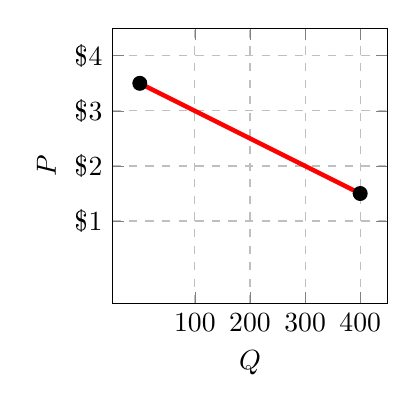
\begin{tikzpicture}[scale=1]
            \begin{axis}[
                %    axis y line = left,
                %    axis x line = bottom,
                    xlabel={$Q$},
                    xtick       = {1,2,3,4},
                    xticklabels = {100,200,300,400},
                    ylabel={$P$},
                    ytick       = {1,2,3,4},
                    yticklabels = {\$1,\$2,\$3,\$4},
                    samples     = 160,
                    domain      = -1:5,
                    restrict y to domain=-1:5,
                    xmin = -0.5, xmax = 4.5,
                    ymin = -0.5, ymax = 4.5,
                    grid=both, grid style=dashed,
                    width=2in, height=2in
                  ]
                  \draw[ultra thick,red] (0,3.5) -- (4,1.5);
                  \filldraw (0,3.5) circle (2.5pt);
                  \filldraw (4,1.5) circle (2.5pt);
            \end{axis}
        \end{tikzpicture}
\end{center}
%\end{minipage}
}


\begin{enumerate}

\item[(b)] What is the {\bf average rate of change} of the price of $1$ unit of the commodity as the quantity demanded changes from $100$ to $300$ units of the commodity?
\sol{
AROC=$\ds \frac{\Delta P}{\Delta Q}=\frac{-1}{300-100}=-\frac{1}{200}$ in \$ per unit.
}
\item[(c)] What is the {\bf slope} of the demand curve? What is the {\bf equation} of the demand curve? (Be sure to indicate the {\bf domain} - that is, to which values of $Q$ your equation pertains.)
\sol{
\itemC{
\item $m$ = Slope = AROC =$\ds -\frac{1}{200}$
\item There are two reasonable approaches to constructing a linear function.
\itemC{
\item {\em Point-Slope} Form.  Choose one point on the graph, say $(Q_1,P_1)=(100,3)$.  Then
\al{
P-P_1&=m(Q-Q_1)\\
P-3&=-\frac{1}{200}(Q-100)\\
P&=-\frac{1}{200}(Q-100)+3
}
\item {\em Slope-Intercept} Form.  Again, choose one point on the graph,  say $(Q_1,P_1)=(100,3)$.  Then
\al{
P&=mQ+b\\
3&=-\frac{1}{200}\cdot 100+b\\
3+\frac{100}{200}&=b\\
3.5&=b\\
P&=-\frac{1}{200}Q+3.5
}
}
\item Domain. There are at least $3$ assumptions students can make that lead to different answers.
\itemI{
\item ``I don't know anything about this demand curve beyond what I see." Thus the domain must be $0\leq Q\leq 400$
\item "The demand curve will continue to the right until the Price hits $0$."  This occurs when $\ds P=-\frac{Q}{200}+3/5=0$.
\al{
-\frac{Q}{200}+3/5&=0\\
-\frac{Q}{200}&=\,-3/5
} 
Thus when I solve for $Q$ I get $Q=700$. Thus the domain  is $0\leq Q\leq 700$.\\\\

\item ``The domain curve will continue to the right and Price can be negative in some cases." Thus the domain is $0 \leq Q < \infty$. \href{https://www.stanwell.com/our-news/energy-explainer/negative-prices/}{\color{red}Here is an example of when negative prices can occur.}
}
}
}
\item[(d)] Write a sentence describing what the slope of the demand curve represents in this context.\\ 
({\bf Note:} ``in this context" means your answer must clearly relate to the scenario described in the problem - a demand curve relating a quantity $Q$ and its unit price $P$. Answers like ``rise over run" are not in-context.)
   \sol{
   The price of the commodity decreases by $\dfrac{1}{200}$ dollars per unit of the commodity when consumers demand an additional unit of the commodity.
   }
\end{enumerate}

\newpage

\,

\vspace{-0.3in}

\minil {\it Average Rate of Change (AROC) vs. Instantaneous Rate of Change (IROC)}\\
% Average rate of change and instantaneous rate of change answer two different questions. Average rate of change can be used to answer a question like "
\mpageT{.48}{.48}[\, \vline \,]{
	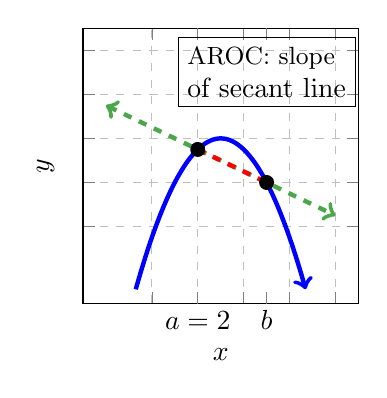
\begin{tikzpicture}[scale=1]
	    \begin{axis}[
	        %    axis y line = left,
	        %    axis x line = bottom,
	            xlabel={$x$},
	            xtick       = {1,2,3,4,5},
	            extra x ticks={ 2, 3.5},
	            extra x tick labels={$a=2$,$b$},
	            extra tick style={grid=none},
	            xticklabels = {},
	            xticklabel  style={yshift=-3ex, anchor=south},
	            ylabel={$y$},
	            ytick       = {1,2,3,4,5},
	            yticklabels = {},
	            samples     = 160,
	            domain      = -1:5,
	            restrict y to domain=-1:5,
	            xmin = -0.5, xmax = 5.5,
	            ymin = -0.75, ymax = 5.5,
	            grid=both, grid style=dashed,
	            width=2in, height=2in
	            ]
	            % curve
	            %\addplot[blue, ultra thick, mark=none, smooth, <->] coordinates{ (0,0) (1,2) (2,3) (3,3) (4,2) (5,.5) };
	            \addplot[blue, ultra thick, mark=none, smooth, domain=0.65:4.35, ->] {3-(x-2.5)^2};
	            \draw[ultra thick, green!50!black!70, dashed, <->] (0,3.75) -- (5,1.25);
	             \draw[ultra thick, red, dashed] (2,2.75) -- (3.5,2);
	            \filldraw (2,2.75) circle (2.5pt);
	            \filldraw (3.5,2) circle (2.5pt);
	            \node[draw, align=left] at (3.5,4.5)  {\small AROC:  slope\\ of secant line};
	    \end{axis}
	\end{tikzpicture}
	\blue{
	\itemI{
	\item The {\em secant} is the  dashed line in connecting the two points on the graph, i.e. for $a\leq x\leq b$
	\item AROC is the {\em  slope} of the secant line.
	\item Interpretation: AROC measure the change in $y$ averaged across the change in $x$ across the {\bf given interval}, $a\leq x \leq b$.
	}
	}
}{
	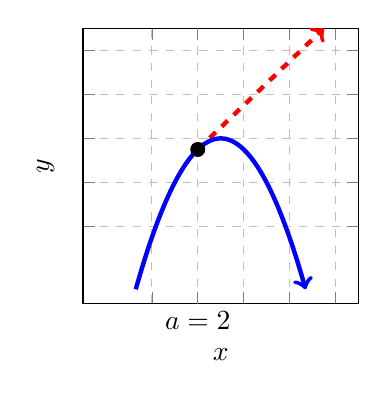
\begin{tikzpicture}[scale=1]
	    \begin{axis}[
	        %    axis y line = left,
	        %    axis x line = bottom,
	            xlabel={$x$},
	            xtick       = {1,2,3,4,5},
	            xticklabels = {},
	             xticklabel  style={yshift=-3ex, anchor=south},
	            extra x ticks={ 2},
	            extra x tick labels={$a=2$},
	            extra tick style={grid=none},
	            ylabel={$y$},
	            ytick       = {1,2,3,4,5},
	            yticklabels = {},
	            samples     = 160,
	            domain      = -1:5,
	            restrict y to domain=-1:5,
	            xmin = -0.5, xmax = 5.5,
	            ymin = -0.75, ymax = 5.5,
	            grid=both, grid style=dashed,
	            width=2in, height=2in
	            ]
	            % curve
	            %\addplot[blue, ultra thick, mark=none, smooth, <->] coordinates{ (0,0) (1,2) (2,3) (3,3) (4,2) (5,.5) };
	            \draw[ultra thick, red, dashed, ->] (2,2.75) -- (4.75,5.5);
	            \addplot[blue, ultra thick, mark=none, smooth, domain=0.65:4.35, ->] {3-(x-2.5)^2};
	            %\addplot[blue, ultra thick, dashed, mark=none, smooth, domain=2:4.35, ->] {3-(x-2.5)^2};
	            \filldraw (2,2.75) circle (2.5pt);
	    \end{axis}
	\end{tikzpicture}
	\blue{
	\itemC{
	\item The {\em instantaneous rate of change},  is the slope of the tangent line at the point on the graph above $x=a$.
	\item IROC is measured {\bf at a point} while AROC is measured {\bf over an interval}
	\item Interpretation: IROC measures how $y$ would change if the function would continue to change exactly as it did in an instant given by a particular $x$-value. In this case $x=a$.
	}
	}
}

\exercise{\color{ProcessBlue}F1} The graph of $y=3-\left(x-\dfrac52\right)^2$ is given in the mini-lecture above. The instantaneous rate of change of $y$ with respect to $x$ in the instant when $x=2$ is $1$. (We will learn how to compute this quantity directly in a few weeks, but for now let's take it as a given.)

\begin{enumerate}
\item[(a)] Find the average rate of change of $y$ as $x$ changes from $2$ to $4$. Then, sketch  a secant line associated with this quantity in the coordinate plane below.\\
%
\mpage{.25}{.75}{
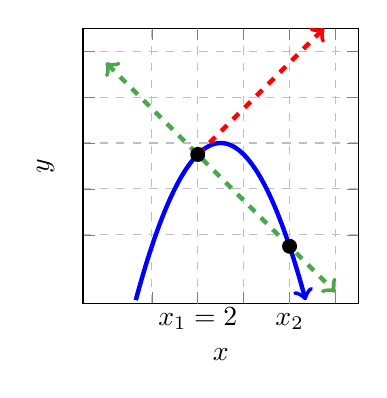
\begin{tikzpicture}[scale=1]
    \begin{axis}[
        %    axis y line = left,
        %    axis x line = bottom,
            xlabel={$x$},
            xtick       = {1,2,3,4,5},
            xticklabels = {},
	xticklabel  style={yshift=-3ex, anchor=south},
             extra x ticks={ 2, 4},
	      extra x tick labels={$x_1=2$,$x_2$},
	      extra tick style={grid=none},
            ylabel={$y$},
            ytick       = {1,2,3,4,5},
            yticklabels = {},
            samples     = 160,
            domain      = -1:5,
            restrict y to domain=-1:5,
            xmin = -0.5, xmax = 5.5,
            ymin = -0.5, ymax = 5.5,
            grid=both, grid style=dashed,
            width=2in, height=2in
            ]
            % curve
            %\addplot[blue, ultra thick, mark=none, smooth, <->] coordinates{ (0,0) (1,2) (2,3) (3,3) (4,2) (5,.5) };
            \addplot[blue, ultra thick, mark=none, smooth, domain=0.65:4.35, ->] {3-(x-2.5)^2};
              \draw[ultra thick, red, dashed, ->] (2,2.75) -- (4.75,5.5);
               	   \draw[ultra thick, green!50!black!70, dashed, <->] (0,4.75) -- (5,-.25); % secant line
		%\draw[ultra thick, red, dashed] (2,2.75) -- (4,.75); %secant
		\filldraw (2,2.75) circle (2.5pt);
               \filldraw (4,.75) circle (2.5pt);
    \end{axis}
\end{tikzpicture}
}{
\sol{
\itemI{
\item $\ds x_1=2\Rightarrow y_1=3-\left(2-\frac{5}{2} \right)^2=3-\left(-\frac{1}{2} \right)^2=3-\frac{1}{4}=2.75$
\item $\ds x_2=4\Rightarrow y_2=3-\left(4-\frac{5}{2} \right)^2=3-\left(\frac{3}{2} \right)^2=3-\frac{9}{4}=0.75$
\item $\ds AROC=\frac{\Delta y}{\Delta x}=\frac{y_2-y_1}{x_2-x_1}=\frac{0.75-2.75}{4-2}=\frac{-2}{2}=-1$
\item Slope of secant line $= AROC = -1$
}
}
}
\newpage
\item[(b)] Find the average rate of change of $y$ as $x$ changes from $2$ to $3.5$. Then, sketch  a secant line associated with this quantity in the coordinate plane below.\\
%
\mpage{.25}{.75}{
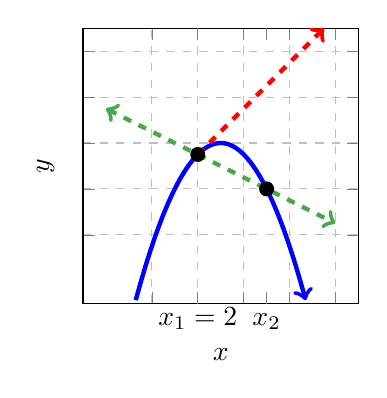
\begin{tikzpicture}[scale=1]
    \begin{axis}[
        %    axis y line = left,
        %    axis x line = bottom,
            xlabel={$x$},
            xtick       = {1,2,3,4,5},
            xticklabels = {},
            	xticklabel  style={yshift=-3ex, anchor=south},
             extra x ticks={ 2, 3.5},
	      extra x tick labels={$x_1=2$,$x_2$},
	      extra tick style={grid=none},
            ylabel={$y$},
            ytick       = {1,2,3,4,5},
            yticklabels = {},
            samples     = 160,
            domain      = -1:5,
            restrict y to domain=-1:5,
            xmin = -0.5, xmax = 5.5,
            ymin = -0.5, ymax = 5.5,
            grid=both, grid style=dashed,
            width=2in, height=2in
            ]
            % curve
            %\addplot[blue, ultra thick, mark=none, smooth, <->] coordinates{ (0,0) (1,2) (2,3) (3,3) (4,2) (5,.5) };
            \addplot[blue, ultra thick, mark=none, smooth, domain=0.65:4.35, ->] {3-(x-2.5)^2};
              \draw[ultra thick, red, dashed, ->] (2,2.75) -- (4.75,5.5);
            	            \draw[ultra thick, green!50!black!70, dashed, <->] (0,3.75) -- (5,1.25);
	          %   \draw[ultra thick, red, dashed] (2,2.75) -- (3.5,2);
	                      \filldraw (2,2.75) circle (2.5pt);
	            \filldraw (3.5,2) circle (2.5pt);
    \end{axis}
\end{tikzpicture}
}{
\sol{
\itemI{
\item $\ds x_1=2\Rightarrow y_1=3-\left(2-\frac{5}{2} \right)^2=3-\left(-\frac{1}{2} \right)^2=3-\frac{1}{4}=2.75$
\item $\ds x_2=3.5\Rightarrow y_2=3-\left(3.5-\frac{5}{2} \right)^2=3-\left(1 \right)^2=3-1=2$
\item $\ds AROC=\frac{\Delta y}{\Delta x}=\frac{y_2-y_1}{x_2-x_1}=\frac{2-2.75}{3.5-2}=\frac{-1.75}{1.5}=-\frac{1}{2}$
\item Slope of secant line $\ds= AROC = -\frac{1}{2}$
}
}
}

\item[(c)] Find the average rate of change of $y$ as $x$ changes from $2$ to $2.5$. Then, sketch  a secant line associated with this quantity in the coordinate plane below.\\
%
\mpage{.25}{.75}{
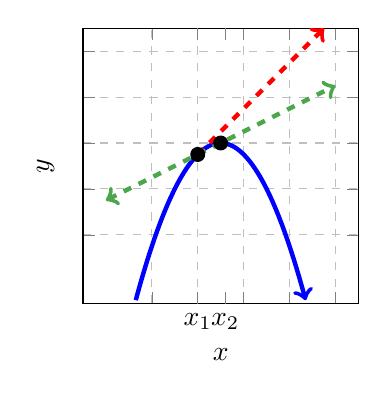
\begin{tikzpicture}[scale=1]
    \begin{axis}[
        %    axis y line = left,
        %    axis x line = bottom,
            xlabel={$x$},
            xtick       = {1,2,3,4,5},
            xticklabels = {},
            	xticklabel  style={yshift=-3ex, anchor=south},
             extra x ticks={ 2, 2.6},
	      extra x tick labels={$x_1$,$x_2$},
	      extra tick style={grid=none},
            ylabel={$y$},
            ytick       = {1,2,3,4,5},
            yticklabels = {},
            samples     = 160,
            domain      = -1:5,
            restrict y to domain=-1:5,
            xmin = -0.5, xmax = 5.5,
            ymin = -0.5, ymax = 5.5,
            grid=both, grid style=dashed,
            width=2in, height=2in
            ]
            % curve
            %\addplot[blue, ultra thick, mark=none, smooth, <->] coordinates{ (0,0) (1,2) (2,3) (3,3) (4,2) (5,.5) };
            \addplot[blue, ultra thick, mark=none, smooth, domain=0.65:4.35, ->] {3-(x-2.5)^2};
              \draw[ultra thick, red, dashed, ->] (2,2.75) -- (4.75,5.5);
		\draw[ultra thick, green!50!black!70, dashed, <->] (0,1.75) -- (5,4.25);
		%\draw[ultra thick, red, dashed] (2,2.75) -- (2.5,3);
		\filldraw (2.5,3) circle (2.5pt);
		            \filldraw (2,2.75) circle (2.5pt);
    \end{axis}
\end{tikzpicture}
}{
\sol{
\itemI{
\item $\ds x_1=2\Rightarrow y_1=3-\left(2-\frac{5}{2} \right)^2=3-\left(-\frac{1}{2} \right)^2=3-\frac{1}{4}=2.75$
\item $\ds x_2=2.5\Rightarrow y_2=3-\left(2.5-\frac{5}{2} \right)^2=3-\left(0 \right)^2=3-0=3$
\item $\ds AROC=\frac{\Delta y}{\Delta x}=\frac{y_2-y_1}{x_2-x_1}=\frac{3-2.75}{2.5-2}=\frac{-0.25}{0.5}=\frac{1}{2}$
\item Slope of secant line $\ds= AROC = \frac{1}{2}$
}
}
}

\item[(d)] Which of our answers to parts (a), (b), and (c) came the closest to the given instantaneous rate of change of $y$ with respect to $x$ in the instant when $x$ is $2$? How could we have predicted this answer would have been the closest before calculating anything?\\
\sol{
Our answer in part c) was closest. It seems that AROC got closer to IROC as the $x$-values got closer to $x_1=2$. This is the same as saying $\Delta x=x_2-x_1$ got smaller towards $0$.  \\
\\
{\em Key takeaway:} As $\Delta x$ approaches $0$, AROC approaches IROC.
}
\vfill
\vfill

\end{enumerate}
\newpage
{\bf\color{blue} Extra Practice.} \reversemarginpar\marginnote{\fbox{\bf\color{ProcessBlue} F1}} The table below provides a sprinter's approximate position (in meters) from the start line at various times (in seconds) after the start of the 100 meter race.

\begin{center}
    \begin{tabular}{| l | l |}
    \hline
    Time (sec) & Distance (m)\\
    \hline
    8 & 81.7\\
    \hline
    8.3 & 85.6\\
    \hline
    8.5 & 88.2\\
    \hline
    8.8 & 91.3\\
    \hline
    9 & 94.1\\
    \hline
    \end{tabular}
\end{center}

We want to know how fast the sprinter was moving exactly $8.5$ seconds after the beginning of the race. 

\begin{enumerate}
\item[(a)] Simplify the following quantity {\bf and} describe what the quantity represents in terms of the context given above:
\sol{
\[ \dfrac{88.2-81.7}{8.5-8} \blue{= \frac{6.5}{0.5}=13} \]
On average, the sprinter traveled $13$ meters per second between $8$ and $8.5$ seconds after the race began.
}


    
\item[(b)]Given the speed of the sprinter is the instantaneous rate of change of position with respect to time, use the data in the table to find 3 different estimates of how fast the sprinter was moving exactly $8.5$ seconds after the beginning of the race.
\sol{
Let's use the variable $t$ to represent time and $D$ to represent Distance.
\enumE{
\item AROC over $t_1=8.5$ to $t_2=8.8$ is $\ds \frac{\Delta D}{\Delta t}=\frac{D_2-D_1}{t_2-t_1}=\frac{91.3-88.2}{8.8-8.5}=\frac{3.1}{0.3}\approx 10.33\;m/sec$
\item AROC over $t_1=8.3$ to $t_2=8.5$ is $\ds \frac{\Delta D}{\Delta t}=\frac{D_2-D_1}{t_2-t_1}=\frac{88.2-85.6}{8.5-8.3}=\frac{2.6}{0.2}= 13.0 \;m/sec$
\item AROC over $t_1=8.5$ to $t_2=9$ is $\ds \frac{\Delta D}{\Delta t}=\frac{D_2-D_1}{t_2-t_1}=\frac{94.1-88.2}{9-8.5}=\frac{5.9}{0.5}= 11.8\;m/sec$
}
Other intervals are also good options. For example $t_1=8.5$ and $t-2=8$ OR $t_1=8.3$ and $t_2=8.8$
}


\item[(c)] Which of your estimates in part (b) is best, and why?
\sol{
We are trying to estimate how fast the sprinter was moving exactly at $8.5$ seconds. Since we want the rate of change exactly at the time $t=8.5$ which means we are looking for IROC. We saw in Exercise C that the smallest change in $x$ ($\Delta x$) produced an AROC that was closest to IROC.  Thus in this example, we are looking for the smallest change in $t$ or $\Delta t$.  Let's go back to our three attempts from (a) to find smallest $\Delta t$
\enumE{
\item $\ds \Delta t=8.8-8.5=0.3$
\item $\ds \Delta t=8.5-8.3=0.2$
\item $\ds \Delta t=9-8.5=0.5$
}
Since \#$2$ has smallest $\Delta t$, it is likely that IROC is around $13\; m/sec$
}

\end{enumerate}

% want them to find slope given a graph, an equation, two points, etc.

% want them to interpret a slope as a rate of change in context

% want them to connect + slope with increasing quantity and - slope with decreasing quantity

% want them to intuit that maximum and minimum values occur where a quantity changes from incr to decr or decr to incr, respectively

\end{document}


%%%%%%%%%%%% F1 Assessment Question %%%%%%%%%%%%%%

\exercise{\bf\color{ProcessBlue}F1} A {\bf supply curve} is a graph depicting the relationship between the quantity $Q$ of a commodity a produce is willing to supply at various prices $P$ of that commodity. The supply curve for a particular commodity is given below.

\begin{center}
        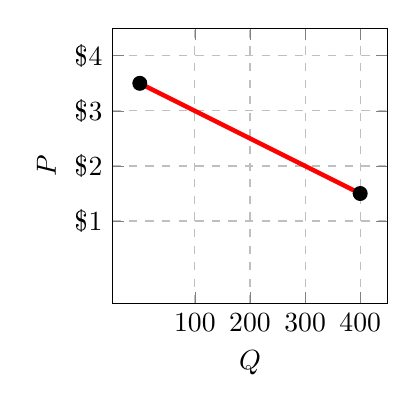
\begin{tikzpicture}[scale=1]
            \begin{axis}[
                %    axis y line = left,
                %    axis x line = bottom,
                    xlabel={$Q$},
                    xtick       = {1,2,3,4},
                    xticklabels = {100,200,300,400},
                    ylabel={$P$},
                    ytick       = {1,2,3,4},
                    yticklabels = {\$1,\$2,\$3,\$4},
                    samples     = 160,
                    domain      = -1:5,
                    restrict y to domain=-1:5,
                    xmin = -0.5, xmax = 4.5,
                    ymin = -0.5, ymax = 4.5,
                    grid=both, grid style=dashed,
                    width=2in, height=2in
                  ]
                  \draw[ultra thick,red] (0,3.5) -- (4,1.5);
                  \filldraw (0,3.5) circle (2.5pt);
                  \filldraw (4,1.5) circle (2.5pt);
            \end{axis}
        \end{tikzpicture}
\end{center}

\begin{enumerate}
\item[(a)] What is the {\bf net change} $\Delta P$ of the price of $1$ unit of the commodity as the quantity supplied changes from $0$ to $300$ units of the commodity?
    \vfill
\item[(b)] What is the {\bf average rate of change} $\dfrac{\Delta P}{\Delta Q}$ of the price of $1$ unit of the commodity as the quantity supplied changes from $0$ to $300$ units of the commodity?
    \vfill
\item[(c)] What is the {\bf slope} of the supply curve? What is the {\bf equation} of the supply curve? Be sure to indicate the {\bf domain} - that is, to which values of $Q$ your equation pertains.
    \vfill
\item[(d)] Write a sentence describing what the slope of the supply curve represents in this context.\\ 
({\bf Note:} ``in this context" means your answer must clearly relate to the scenario described in the problem - a supply curve relating a quantity $Q$ and its unit price $P$. Answers like ``rise over run" are not in this context.)
    \vfill
\end{enumerate}



%%%%%%%%% Unused Exercise %%%%%%%%%

\exercise{\bf\color{ProcessBlue}F1} A {\bf supply curve} is a graph depicting the relationship between the quantity $Q$ of a commodity a produce is willing to supply at various prices $P$ of that commodity. The supply \& demand curves for a particular commodity is given below.

\begin{center}
        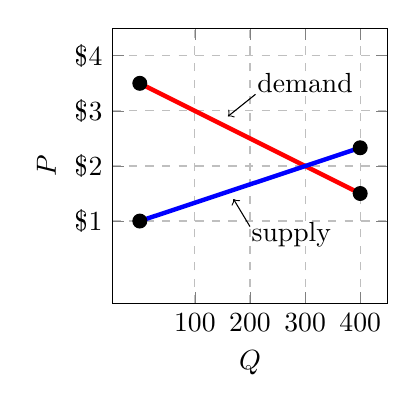
\begin{tikzpicture}[scale=1]
            \begin{axis}[
                %    axis y line = left,
                %    axis x line = bottom,
                    xlabel={$Q$},
                    xtick       = {1,2,3,4},
                    xticklabels = {100,200,300,400},
                    ylabel={$P$},
                    ytick       = {1,2,3,4},
                    yticklabels = {\$1,\$2,\$3,\$4},
                    samples     = 160,
                    domain      = -1:5,
                    restrict y to domain=-1:5,
                    xmin = -0.5, xmax = 4.5,
                    ymin = -0.5, ymax = 4.5,
                    grid=both, grid style=dashed,
                    width=2in, height=2in
                  ]
                  % demand
                  \draw[ultra thick,red] (0,3.5) -- (4,1.5);
                  \filldraw (0,3.5) circle (2.5pt);
                  \filldraw (4,1.5) circle (2.5pt);
                  \node at (3,3.5) {demand};
                  \draw[->] (2.1,3.3) -- (1.6,2.9);
                  % supply
                  \draw[ultra thick, blue] (0,1) -- (4,2.33);
                  \filldraw (0,1) circle (2.5pt);
                  \filldraw (4,2.33) circle (2.5pt);
                  \node at (2.75,.75) {supply};
                  \draw[->] (2,.9) -- (1.7,1.4);
            \end{axis}
        \end{tikzpicture}
\end{center}

\begin{enumerate}
    \item[(a)] Find the slopes of the given supply \& demand curves.

    \begin{center}
    {\Large $m_{\text{supply}}=$\rule[-8pt]{0.5in}{0.4pt} \quad $m_{\text{demand}}=$\rule[-8pt]{0.5in}{0.4pt}}
    \end{center}
    
    \item[(b)] Assuming $P$ is a function of $Q$, we say $P$ is an {\bf increasing} function of $Q$ if $P$ increases as $Q$ increases, and we say $P$ is a {\bf decreasing} function of $Q$ if $P$ decreases as $Q$ increases.\\[0.05in]
    Along the supply curve, is unit price $P$ an increasing or decreasing function of quantity $Q$? Along the demand curve, is unit price $P$ an increasing or decreasing function of quantity $Q$? (circle appropriately below)

    \vspace{-0.3in}

    {\Large
    \begin{align*}
    \text{supply: } &&P \text{ is an} &&\text{increasing} &&/ &&\text{decreasing} &&\text{function of }Q\\[0.1in]
    %
    \text{demand: } &&P \text{ is an} &&\text{increasing} &&/ &&\text{decreasing} &&\text{function of }Q
    \end{align*}
    }

    \item[(c)] How can we decide using only the slopes of the supply \& demand curves whether $P$ is an increasing or decreasing function of $Q$? Explain.

    \vfill

\end{enumerate}